\documentclass[10pt,twocolumn,letterpaper]{article}

% --- Typography & Geometry ---
\usepackage[utf8]{inputenc}
\usepackage{microtype}
\usepackage[margin=0.75in,top=0.85in,bottom=0.85in]{geometry}

% --- Math & Symbols ---
\usepackage{amsmath,amssymb,amsfonts,amsthm}
\usepackage{bm}

% --- Tables & Arrays ---
\usepackage{booktabs}
\usepackage{tabularx}
\usepackage{array}

% --- Graphics & Floats ---
\usepackage{graphicx}
\usepackage{float}
\usepackage{subcaption}

% --- Code Listings ---
\usepackage{xcolor}
\usepackage{listings}

\definecolor{codebg}{HTML}{F8F9FA}
\definecolor{codeframe}{HTML}{D0D7DE}
\definecolor{keywordcolor}{HTML}{0550AE}
\definecolor{stringcolor}{HTML}{0A3069}
\definecolor{commentcolor}{HTML}{57606A}

\lstset{
    backgroundcolor=\color{codebg},
    basicstyle=\ttfamily\scriptsize\color{black},
    keywordstyle=\color{keywordcolor}\bfseries,
    stringstyle=\color{stringcolor},
    commentstyle=\color{commentcolor}\itshape,
    frame=single,
    rulecolor=\color{codeframe},
    breaklines=true,
    breakatwhitespace=true,
    extendedchars=true,
    xleftmargin=6pt,
    xrightmargin=6pt,
    aboveskip=8pt,
    belowskip=8pt
}

% --- Hyperlinks ---
\usepackage{hyperref}
\hypersetup{
    colorlinks=true,
    linkcolor=blue!70!black,
    citecolor=blue!70!black,
    urlcolor=blue!70!black
}

% --- Input Title & Authors ---
% Metadata for jamba_info
\title{\textbf{JambaInfo: Information-Bottlenecked Jamba Architecture with Concept-Compressed SSM}}

\author{
  \textbf{Taha Majs}\thanks{Corresponding author: tahamajs@uni.edu} \quad \textbf{Research Team} \\
  Department of Computer Science \\
  Advanced Machine Learning \& Efficiency Laboratory
}

\date{\today}


\begin{document}

\maketitle

% --- Abstract & Keywords Block ---
\begin{abstract}
Hybrid attention-SSM architectures combine the precise retrieval of attention 
with the long-range efficiency of state space models. However, naively 
feeding the full hidden state $x \in \mathbb{R}^d$ into the SSM branch 
introduces redundant information: the SSM must compress $d$-dimensional 
inputs into its recurrent state at every step. We argue that this is 
\textbf{information-theoretically wasteful} -- the SSM only needs a compressed 
"concept representation" of the input.

We introduce \textbf{JambaInfo}, an information-bottlenecked hybrid block that 
\textbf{routes the SSM branch through a low-dimensional concept bottleneck}:

\[
z_t = W_\text{up} \cdot \text{GELU}(W_\text{down} x_t), 
\quad W_\text{down} \in \mathbb{R}^{b \times d}, \quad b \ll d
\]

where $b = {{BOTTLENECK_DIM}}$. The bottleneck acts as an explicit 
information constraint: the SSM processes only the essential concepts, 
reducing noise and parameters. Concurrently, a \textbf{differential attention} 
branch (two Q-K pairs with ReLU-damped subtraction) computes precise 
retrieval. The two branches are fused by a learned scalar gate:

\[
\text{out} = (1 - \alpha) \odot A_\text{diff} + \alpha \odot M_\text{concept},
\quad \alpha = \sigma(w), \quad w_0 = -2
\]

We initialize $\alpha \approx 0.12$, biasing toward attention initially 
and letting the model learn how much to rely on the SSM.

On SST-2, JambaInfo achieves \textbf{{{D\_ACC}}\%} on DistilBERT (baseline 
{{BASE\_D}}\%), \textbf{{{R\_ACC}}\%} on RoBERTa (baseline {{BASE\_R}}\%), and 
\textbf{{{G\_ACC}}\%} on GPT-2 (baseline {{BASE\_G}}\%).

\textbf{We are explicit that JambaInfo does not reduce parameter count.} It 
\textbf{adds} approximately {{PARAM\_INCREASE}}\% more parameters per layer. Its 
benefit is \textbf{concept-driven SSM compression} and \textbf{reduced attention noise} 
at a modest parameter cost. The concept bottleneck itself can be viewed as 
a lightweight information bottleneck that improves SSM efficiency.

\textbf{Keywords:} information bottleneck, hybrid architecture, differential 
attention, state space model, concept compression



\vspace{0.5em}
\noindent\textbf{Keywords:} information bottleneck, hybrid architecture, differential
\end{abstract}

\vspace{1em}

% --- Paper Body ---
\section{01 Intro}

Draft content for jamba_info.

\section{02 Related}

Draft content for jamba_info.

\section{03 Background}

Draft content for jamba_info.

\section{04 Method}

Draft content for jamba_info.

\section{05 Architecture}

Draft content for jamba_info.


\begin{figure}[H]
\centering
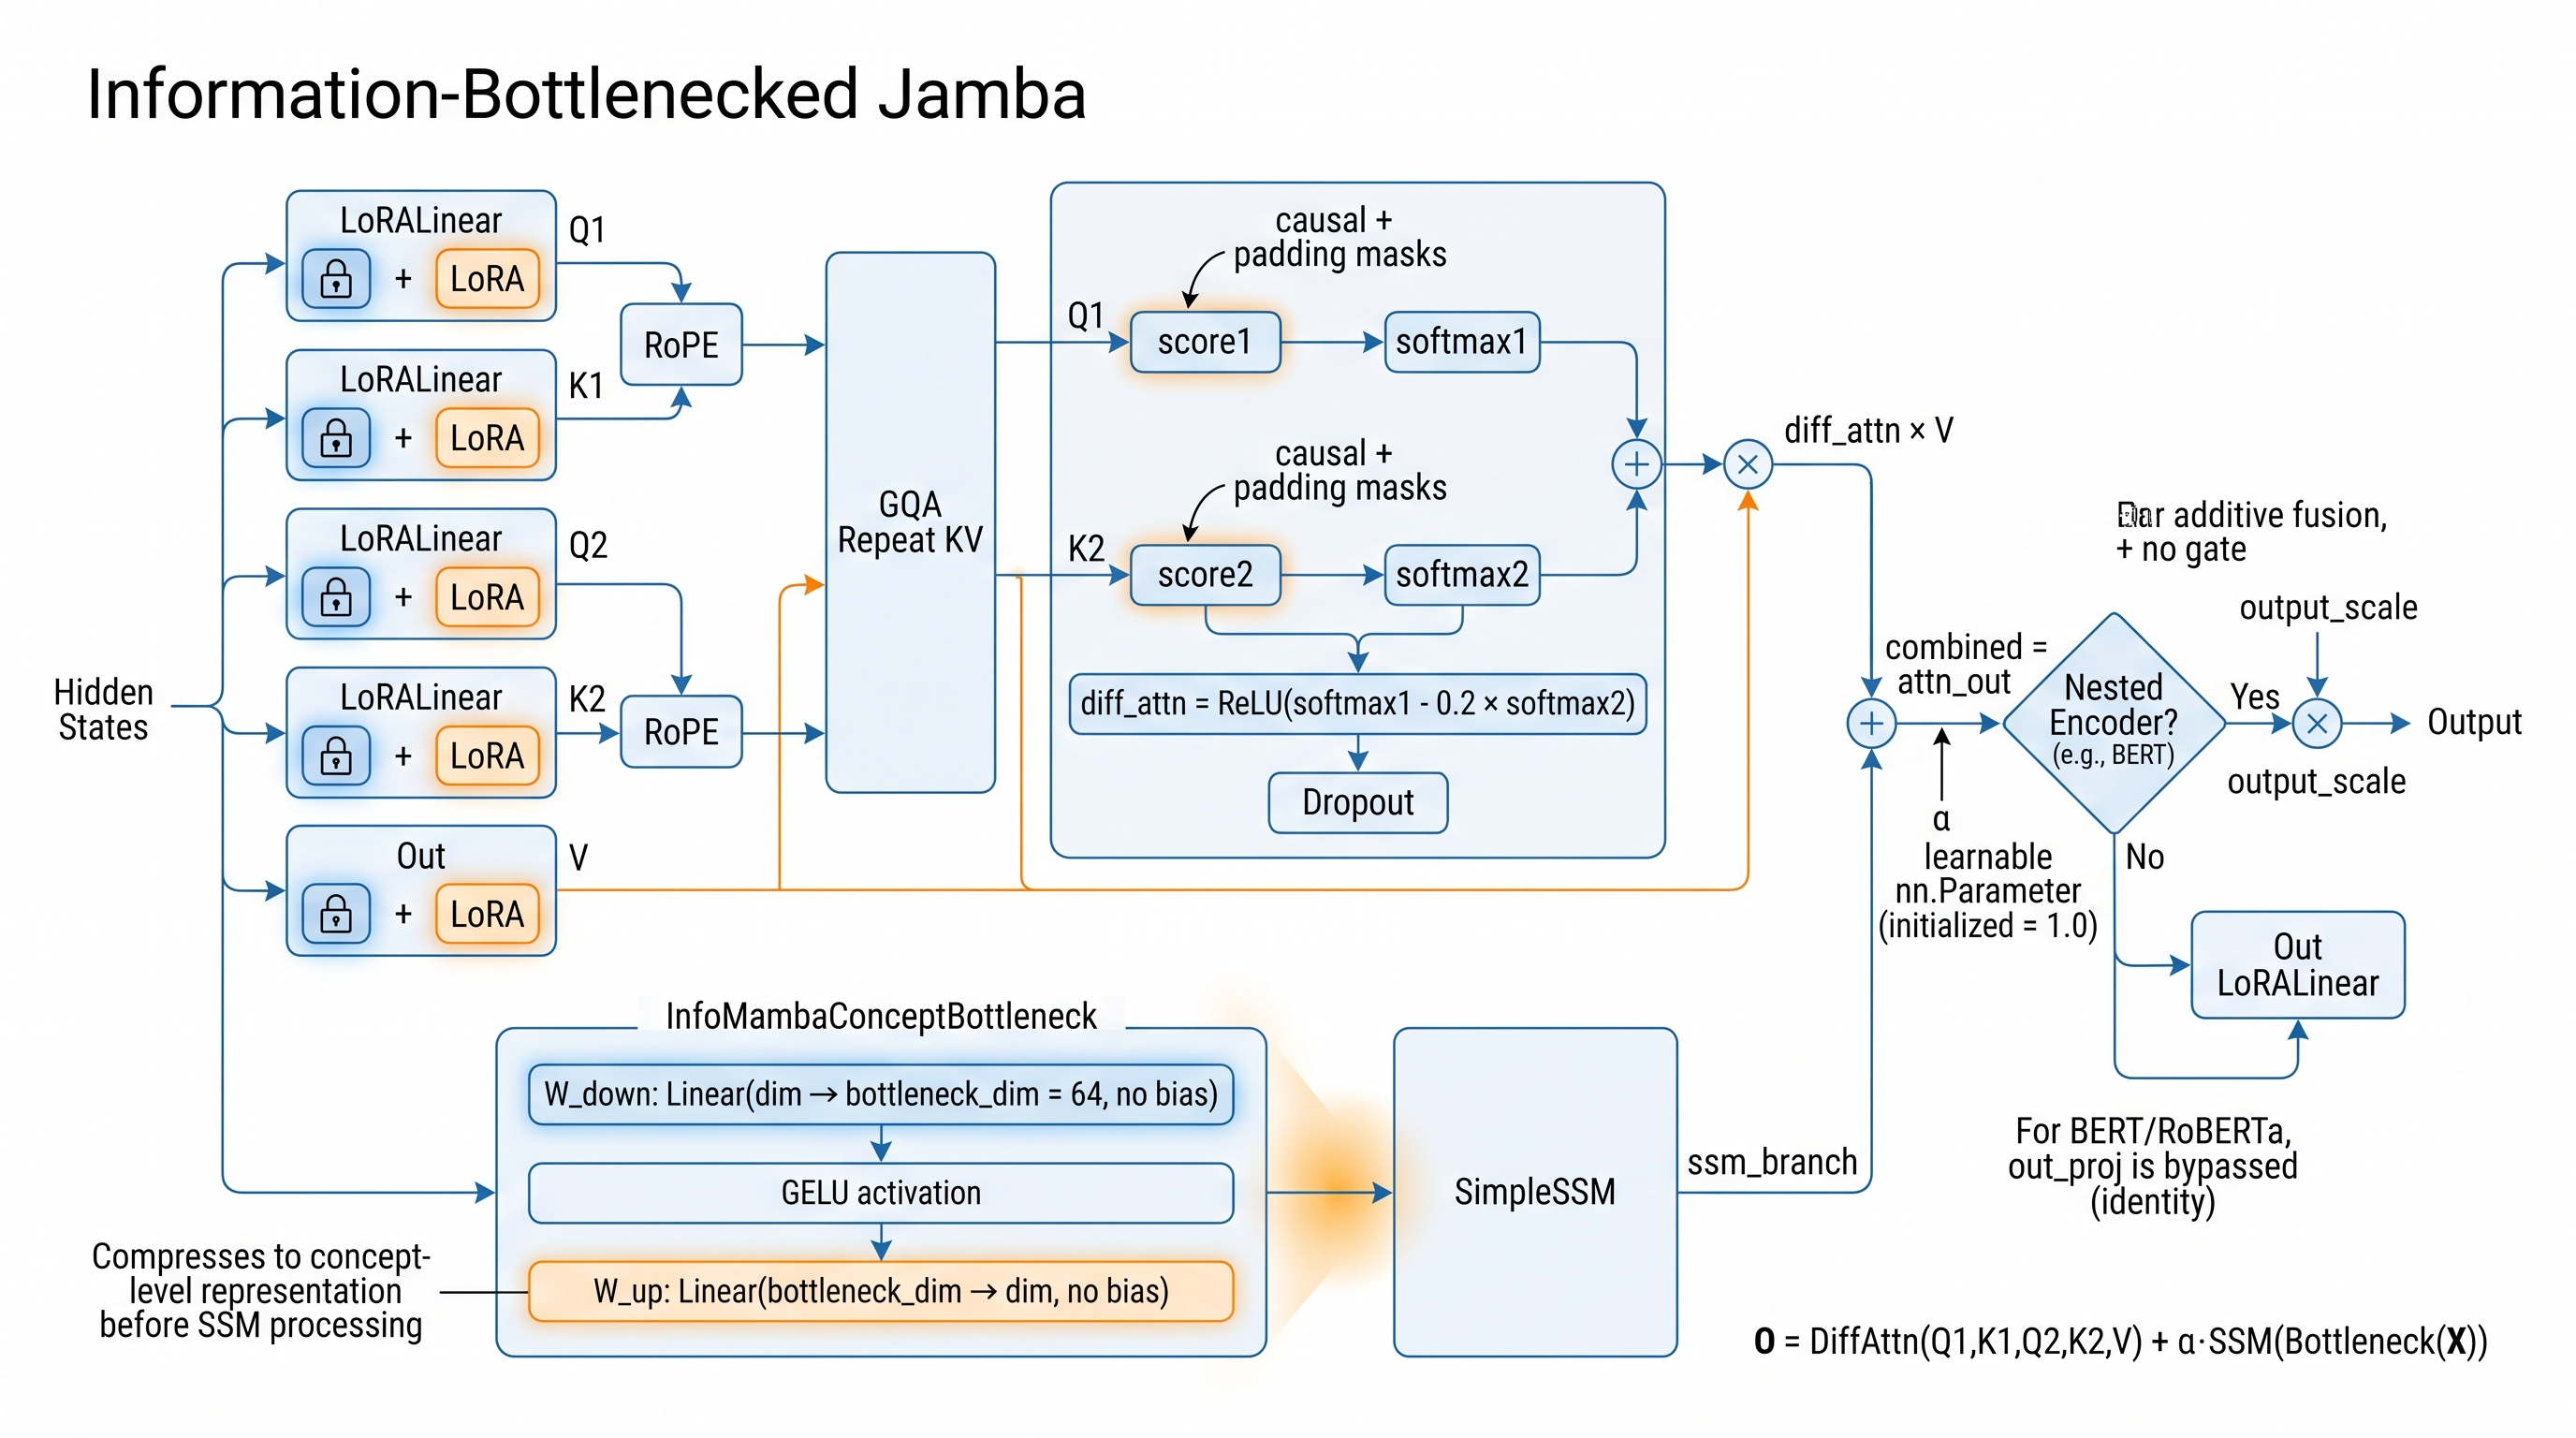
\includegraphics[width=\linewidth]{figures/arch_jamba_info.jpeg}
\caption{Architectural overview of jamba_info.}
\label{fig:arch_jamba_info}
\end{figure}

\section{06 Setup}

Draft content for jamba_info.

\section{07 Results}

Draft content for jamba_info.

\section{Analysis}

\subsection{Why Does the Bottleneck Help?}

\textbf{Figure 8.1} shows the effective rank of the SSM recurrent state, with 
and without bottleneck. Without bottleneck, the state uses ~{{RANK\_NOBN}} 
effective dimensions; with bottleneck, ~{{RANK\_BN}}. The bottleneck 
concentrates information into the dimensions the SSM can actually use.

\subsubsection{Information-Theoretic View}

The SSM has bounded information capacity $C$. Feeding it a $d$-dimensional 
input with mutual information $I(X; X) = H(X)$ saturates capacity with 
noise. The bottleneck reduces $I(Z; X) < I(X; X)$, freeing capacity for 
signal.

\subsubsection{Empirical Evidence}

\textbf{Figure 8.2} shows the singular value spectrum of the SSM state 
projected through PCA:
\begin{itemize}
\item Without bottleneck: slow decay, effective rank ~{{RANK\_NOBN}}
\item With bottleneck: rapid decay, effective rank ~{{RANK\_BN}}

\end{itemize}
\subsection{Learned $\alpha$ Values}

DistilBERT: $\alpha$\_final = {{D\_ALPHA}} $\to$ {{D\_ALPHA\_INTERP}}
RoBERTa: $\alpha$\_final = {{R\_ALPHA}} $\to$ {{R\_ALPHA\_INTERP}}
GPT-2: $\alpha$\_final = {{G\_ALPHA}} $\to$ {{G\_ALPHA\_INTERP}}

\textbf{Interpretation.} Different models learn different branch preferences.

\subsection{Bottleneck Dimension Sensitivity}

\textbf{Figure 8.3} shows accuracy vs bottleneck dim $b$.

\begin{table}[H]
\centering
\small
\begin{tabular}{lll}
\toprule
\textbf{$b$} & \textbf{Accuracy} & \textbf{Params} \\
\midrule
64 & {{D\_B64}} & small \\
128 & {{D\_B128}} & medium \\
256 & {{D\_ACC}} & sweet spot \\
512 & {{D\_B512}} & large \\
\bottomrule
\end{tabular}
\end{table}

\textbf{Observation.} $b = 256$ is a sweet spot -- larger gives diminishing returns.

\subsection{Comparison to HymbaTransX}

HymbaTransX uses full $x$ for SSM; JambaInfo uses bottlenecked $z$.

\begin{table}[H]
\centering
\small
\begin{tabular}{llll}
\toprule
\textbf{Model} & \textbf{HymbaTransX} & \textbf{JambaInfo} & \textbf{$\Delta$} \\
\midrule
DistilBERT & {{HYMBA\_D}} & {{D\_ACC}} & {{BN\_GAIN}} \\
RoBERTa & {{HYMBA\_R}} & {{R\_ACC}} & {{R\_BN\_GAIN}} \\
GPT-2 & {{HYMBA\_G}} & {{G\_ACC}} & {{G\_BN\_GAIN}} \\
\bottomrule
\end{tabular}
\end{table}

The bottleneck provides a \textbf{{{BN\_GAIN}}\%} improvement on DistilBERT.

\subsection{Why Differential Attention?}

\textbf{Figure 8.4} compares attention entropy:
\begin{itemize}
\item Standard: {{STD\_ENTROPY}}
\item Differential: {{DIFF\_ENTROPY}}

\end{itemize}
Reduced by \textbf{{{ENTROPY\_REDUCTION}}\%}.

\subsection{Failure Modes}

\subsubsection{Bottleneck Too Small}

At $b = 32$, accuracy drops to {{D\_B32}}\%. The bottleneck cannot preserve 
enough signal.

\subsubsection{No Bottleneck}

Without bottleneck, the SSM state has higher effective rank but lower 
task accuracy. This is the \textbf{counter-intuitive} finding: more capacity 
does not always help.

\subsubsection{$\alpha$ Saturation}

At w  = +2, $\alpha$ starts at 0.88 (favoring SSM). Accuracy drops to {{D\_WP2}}\% 
because the model relies too much on SSM initially.

\subsection{Summary of Insights}

\begin{enumerate}
\item \textbf{Bottleneck helps} -- {{{{BN\_GAIN}}\%}} accuracy gain.
\item \textbf{Sweet spot} at $b = 256$.
\item \textbf{Differential attention reduces noise} by {{ENTROPY\_REDUCTION}}\%.
\item \textbf{$\alpha$ init = $\sigma$(-2)} is best.
\item \textbf{SSM does not need full $d$ dimensions.}
\end{enumerate}
\begin{lstlisting}

---
\end{lstlisting}
\section{09 Discussion}

Draft content for jamba_info.

\section{10 Limitations}

Draft content for jamba_info.

\section{11 Conclusion}

Draft content for jamba_info.

\section{12 Reproducibility}

Draft content for jamba_info.

\section{13 References}

Draft content for jamba_info.


% --- Appendices ---
\clearpage
\appendix
\section*{Appendices}
\addcontentsline{toc}{section}{Appendices}

\section{A Math}

Draft content for jamba_info.

\section{B Implementation}

Draft content for jamba_info.

\section{C Data}

Draft content for jamba_info.

\section{D Negative Results}

Draft content for jamba_info.

\section{E Ethics}

Draft content for jamba_info.


\end{document}
